\documentclass[parskip,10pt,abstracton]{scrartcl}
\usepackage[top=3cm, bottom=3cm, left=3cm, right=3cm]{geometry}
\usepackage{polyglossia}
\setmainlanguage{german}
%\pagenumbering{gobble}

\usepackage{setspace}
\onehalfspacing

% ------------------------------------------------------------------------------------
% packages
\usepackage[hidelinks]{hyperref}
\usepackage{graphicx}
\usepackage{tikz}
\usetikzlibrary{arrows,shapes,positioning, shadows,trees}
\usepackage{enumerate}

\usepackage{xcolor}

\newcommand{\sbt}{\begin{picture}(-1,1)(-1,-3)\circle*{3}\end{picture}\ } % Punkt


% ------------------------------------------------------------------------------------
% Header
% ------------------------------------------------------------------------------------
\renewcommand*{\maketitle}{%
	\begin{flushright}
	{\rmfamily WiSe 16/17 \par}
	\end{flushright}
	\vspace{-1.3cm}
	
	{\bfseries\sffamily User-Interface Design} \\
	{\rmfamily Tamar Arndt \\ Jens-Christan Foerster \\ Velat Gümüs \par}
	
	{\centering\LARGE\sffamily\bfseries Dokumentation: Kochbuchwebseite \par}
   % {\centering\sffamily \textcolor{red}{Dieses Dokument enthält nur die Aufgaben 6-10, um die Kompilierzeit zu reduzieren.}\par}
	\vspace{1em}
}

%\renewcommand{\thesection}{}
% ====================================================================================
% Document
% ====================================================================================
\begin{document}

\maketitle

\tableofcontents
\newpage

% ------------------------------------------------------------------------------------
% AUFGABE 1
% ------------------------------------------------------------------------------------
\section{Projektidee}

\subsection*{a) Überblick}

Die Idee für das Projekt ist eine \textit{Kochbuch-Webseite} zu erstellen, die für die im folgenden beschriebene Zielgruppe das Zubereiten von Gerichten erleichtern soll.

\textbf{Inhalt}\\
Die Seite bietet eine Sammlung von Rezepten aller Art.
Die Rezepte sind in verschiedene Kategorien eingeordnet und können sortiert und durchsucht werden.
Nutzer können Rezepte bewerten, hinzufügen, kommentieren und ein eigenes digitales Kochbuch verwalten, in dem sie sich Rezepte speichern.
Innerhalb der Rezepte gibt es zu ausgewählten Techniken und Angaben Hinweise für unerfahrene Köche. Der Nutzer kann z.B. eine Erklärung dazu erhalten, was eine Prise Salz ist.

\textbf{Zielgruppe}\\
Zu der Zielgruppe gehören 16 bis 40 jährige Gelegenheitsköche, die der digitalen Version eines Kochbuchs offen gegenüberstehen.
Einerseits spricht die Seite unerfahrene Köche an, die sich über Rezepte und bestimmte Techniken informieren wollen. Andererseits ist die Seite geeignet für inspirationssuchende Gelegenheitsköche, die ein Rezept für einen bestimmten Anlass suchen. Erfahrene Köche haben die Möglichkeit, neue Rezepte zu finden, diese zu speichern und schnell darauf zuzugreifen. 

\textbf{Ziele} \\
Eine der beiden Hauptfunktionen der Webseite ist diese zu nutzen, um sich von den gegebenen Rezepten inspirieren zu lassen. Eine andere Hauptfunktion besteht darin, die Webseite nach bestimmten Rezepten zu durchsuchen. 

% Notizen:
%Features: \\
%- Rezepte merken (eigene Rezeptsammlung erstellen)  $\to$ login \\
%- Rezepte hinzufügen \\
%- kategorisieren / taggen $\to$ Schlagwörter vorschlagen \\
% - suchfunktion \\
% - Tipps (Hinweise zu Techniken) \\
% 
% Zielgruppe: \\
% alle die gerne Kochen \\
% leicht Technikaffin - keine Angst vor digitalen Kochbüchern \\
% 16 - 40 Jahre
% 
% Inspirations suchende \\
% Kochneulinge \\
% auch erfahrene, die ihre Rezepte speichern und schnell wieder finden wollen \\
% Gelegenheitsköche/bäcker, die nur zu bestimmten Anlass etwas brauchen -> Geburtstagskuchen

\subsection*{b) Szenarien}

\begin{enumerate}[(1)]
 \item Max ist 16 Jahre alt (Schüler) und verbringt nicht viel Zeit in der Küche, möchte aber vor Weihnachten Plätzchen backen. Er verwendet die Suchfunktion, um schnell Rezepte für Plätzchen zu finden. Von einigen sieht er sich die Bilder und Kommentare an und entscheidet sich für ein einfaches Rezept.
 
 %Plätzchen backen, sonst kein Vielkocher $\to$ Suchfunktion oder über Kategoriennavigation \\ 16 jährige Schülerin
 
 \item Karl ist Student und hat Hunger. Er hat aber nur Nudeln, Hackfleisch und Tomaten zuhause. Auf der Webseite gibt er diese Zutaten ein und erhält eine kleine Auswahl von Rezepten. 
 
 %Kochen nach Zutaten die zur Verfügung stehen - Rezept finden $\to$ verwendet Suchfunktion nach Zutat \\ fauler Student (oder WG)
 
 \item Anna ist 40 und Hausfrau. Sie möchte am Sonntag für ihre Familie ein neues Rezept ausprobieren. Auf der Webseite klappt sie das Seitenmenü ein und scrollt durch die Bilder. Sie öffnet ein Rezept, das ihr gefällt. Danach speichert sie das Rezept ab und betrachtet ihre gespeicherten Rezepte. 
 
 %Inspirationssuchender $\to$ verwendet Merkfunktion \\ Hausfrau ca 40, will neues ausprobieren
\end{enumerate}



\definecolor{inhalt}{HTML}{A1D490}
\definecolor{rahmen}{HTML}{ABBEC4}
% ------------------------------------------------------------------------------------
% AUFGABE 2
% ------------------------------------------------------------------------------------
\section{Navigationsstruktur}


\textbf{kurze Erklärung:}\\
Der erste Navigationspunkt unserer Webseite ist Home/Startseite, von der ein Zugriff auf alles weitere möglich ist.

Unsere Webseite soll folgende Inhalte beinhalten:\\
Verschiedene Rezepte geordnet nach vegan, vegetarisch, Fleisch- und Fischgerichte, Gemüsegerichte und Länderspäzifische Gerichte. \\
Des Weiteren sind Backrezepte wie Plätzchen, Kuchen, Auflauf, aber auch andere süße oder herzhafte Rezepte zu finden. \\
Außerdem werden es vermutlich Rezepte für Soßen, Dips, Knabberzeug, Salate und Teiggerichte auf der Webseite zu finden sind. 

Deshalb sind die angehenden Stichpunkte auch als Kategorien zu finden. 

Des Weiteren wird es verschiedene Techniken zur Zubereitung von Gerichten geben. 
Zudem wird es einen persönlichen Bereich mit einer Login-Funktion geben, in der Rezepte gespeichert und verwaltet werden können.



\textbf{Inhalte in Oberbegriffen zusammengefasst:} \\
Home | Kochen | Backen | meine Rezepte

Der Bereich 'Techniken' ist in alle Rezept-Unterseiten integriert, also kein eigenständiger Navigationsbereich.

\pagebreak
\textbf{Schema zur Organisation der Begriffe:}\\
Hierarchische Struktur

% Navigationsstruktur
% ---------------------------------------
\tikzset{
  basic/.style  = {draw, rounded corners=2pt, text width=2cm, font=\sffamily, rectangle, text height = 1em, align=center},
  root/.style   = {basic, thin, align=center},
  level 2/.style = {basic, thin,align=center,text width=8em},
  level 3/.style = {basic, thin, align=left, text width=6.5em}
}

\begin{tikzpicture}[
  level 1/.style={sibling distance=40mm},
  edge from parent/.style={-,draw},
  >=latex]

\node[root] {Kochbuch}
  child {node[level 2,fill=rahmen] (c1) {Home}}
  child {node[level 2,fill=inhalt] (c2) {Kochen}}
  child {node[level 2,fill=inhalt] (c3) {Backen}}
  child {node[level 2,fill=rahmen] (c4) {persönl. Bereich}};

\begin{scope}[every node/.style={level 3}]

\node [below of = c2, xshift=15pt,fill=inhalt] (c21) {vegan};
\node [below of = c21,fill=inhalt] (c22) {italienisch};
\node [below of = c22,fill=inhalt] (c23) {Suppe};
\node [below of = c23,fill=inhalt] (c24) {$\cdots$};

\node [below of = c3, xshift=15pt,fill=inhalt] (c31) {Kuchen};
\node [below of = c31,fill=inhalt] (c32) {Kleingebäck};
\node [below of = c32,fill=inhalt] (c33) {$\cdots$};

\node [below of = c4, xshift=15pt,fill=rahmen] (c41) {Login/Logout};
\node [below of = c41,fill=rahmen] (c42) {eigene Rezepte};
\node [below of = c42,fill=rahmen] (c43) {Einstellungen};
\end{scope}

% lines
\foreach \value in {1,...,4}
  \draw[-] (c2.195) |- (c2\value.west);
\foreach \value in {1,...,3}
  \draw[-] (c3.195) |- (c3\value.west);
\foreach \value in {1,...,3}
  \draw[-] (c4.195) |- (c4\value.west);
\end{tikzpicture}

\colorbox{inhalt}{Inhaltlich/Rezepte}\\
\colorbox{rahmen}{Rahmen / äußere Struktur / Organisatorisches}

% ---------------------------------------

Für die Webseite eignet sich eine hierarchische Struktur.
Die Hauptbereiche sind Home, Kochen, Backen und der persönliche Bereich. 

Home ist die Startseite.\\
Kochen und Backen sind jeweils in Unterkategorien aufgedröselt, die zu den jeweiligen Rezepten führen. \\
Der persönliche Bereich ist einerseits die Login-Funktion und andererseits der Bereich für eigene Rezepte.
%Parallel zu dieser Struktur gibt es den persönlichen
%Der persönliche Bereich ist aufgeteilt in den Login und


% ------------------------------------------------------------------------------------
% AUFGABE 3
% ------------------------------------------------------------------------------------
\section{Strukturierung der Nutzeroberfläche}


% ------------------------------------------------------------------------------------
\section*{Entwurf 1} % Chris 1

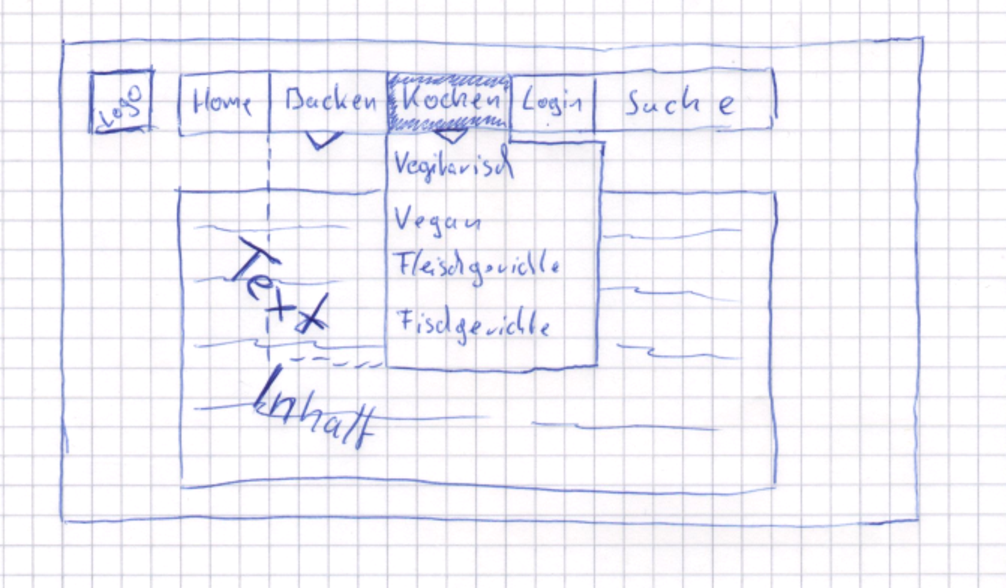
\includegraphics[scale=0.8]{Entwürfe/chris1.pdf}


\textbf{Vorteile:} \\
- einfach und übersichtlich\\
- Seite nicht überladen\\
- viel Platz für Inhalt

\textbf{Nachteile:} \\
- Menüpunkte Backen/Kochen können unübersichtlich werden bei zu vielen Unterkategorien\\
- unklar, was Login beinhaltet (welche Funktionen hat man davon?) $\to$ Hinweis auf persönliche Funktionen / Möglichkeiten

% ------------------------------------------------------------------------------------
\section*{Entwurf 2} % Chris 2

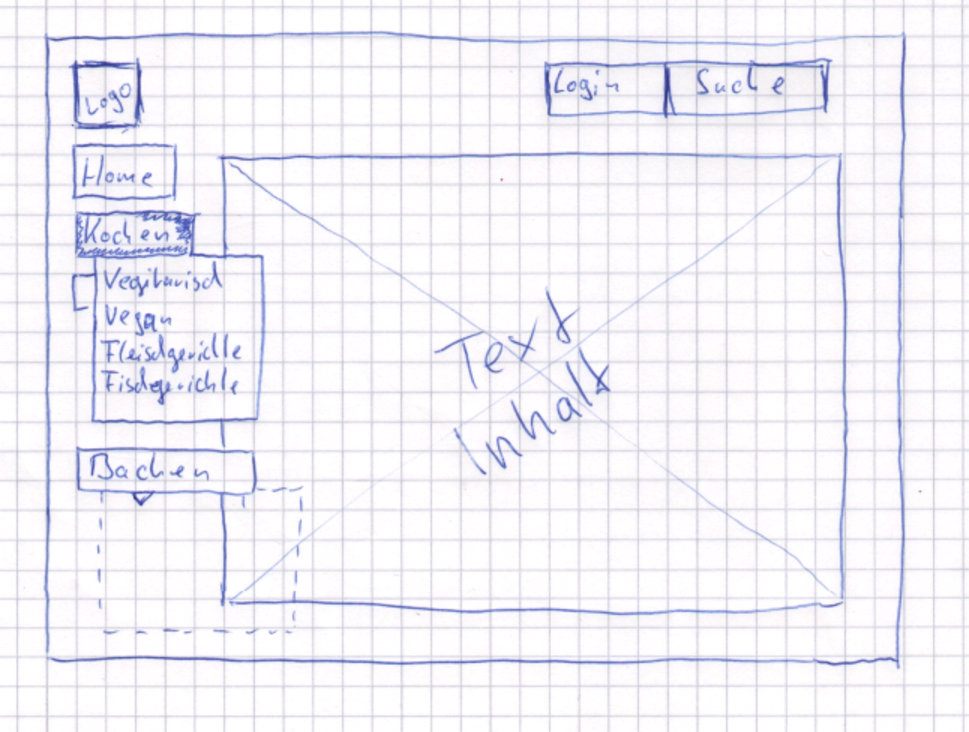
\includegraphics[scale=0.8]{Entwürfe/chris2.pdf}

\textbf{Vorteile:}\\
- klassischer Aufbau und daher intuitives Zurechtfinden möglich (Position von Login und Suche) \\
- übersichtliches Menü, das sich anpasst (Ein- und Ausklappen möglich).
-

\textbf{Nachteile:}\\
- Seitenmenü kann problematisch werden, wenn Menüpunkte zu lang sind.\\
- nicht innovativ, da es sehr oft verwendet wird.


% ------------------------------------------------------------------------------------
\section*{Entwurf 3} % Velat 1

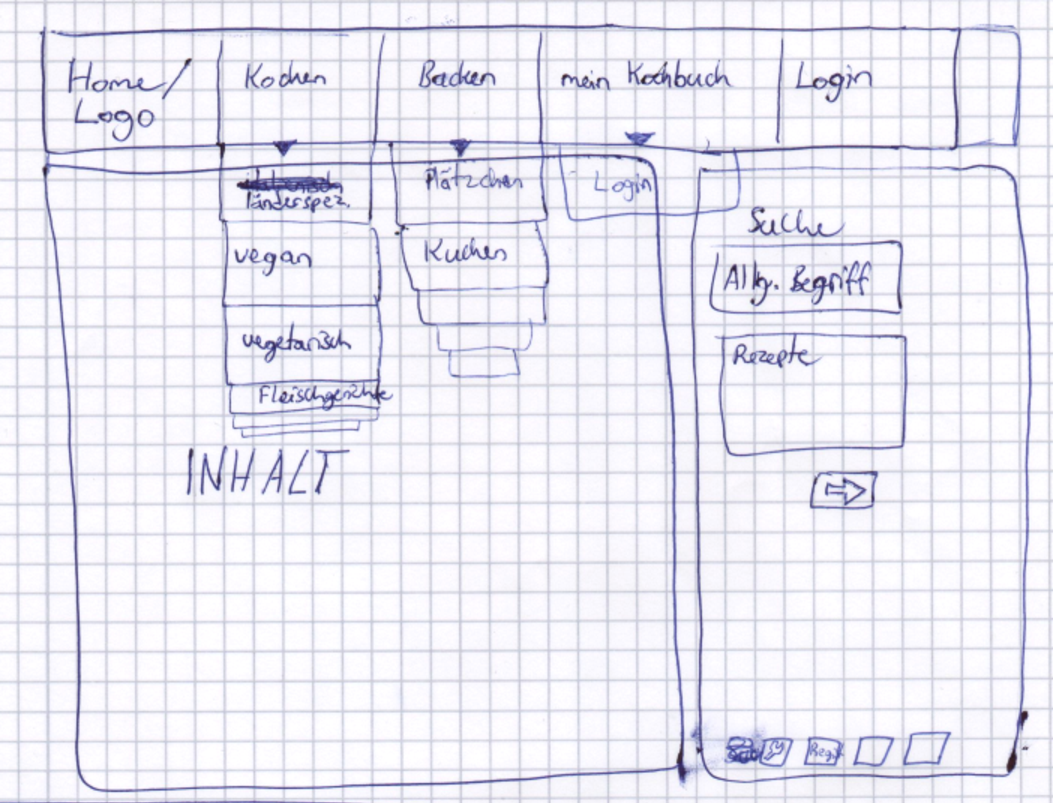
\includegraphics[scale=0.8]{Entwürfe/velat1.pdf}


\textbf{Vorteile:}\\
- es ist ersichtlich, dass es einen eigenen Kochbuchbereich gibt, für den man sich einloggen muss.\\
- innovativer Suchbereich\\
- Suchbereich als eigener Frame jederzeit sichtbar


\textbf{Nachteile:}\\
- Menüpunkte haben zu viele Unterpunkte im Dropdownmenü\\
- Suchbereich verbraucht Platz von Inhaltsseite\\
- Suchfunktion zu kompliziert

% ------------------------------------------------------------------------------------
\section*{Entwurf 4} % Velat 2

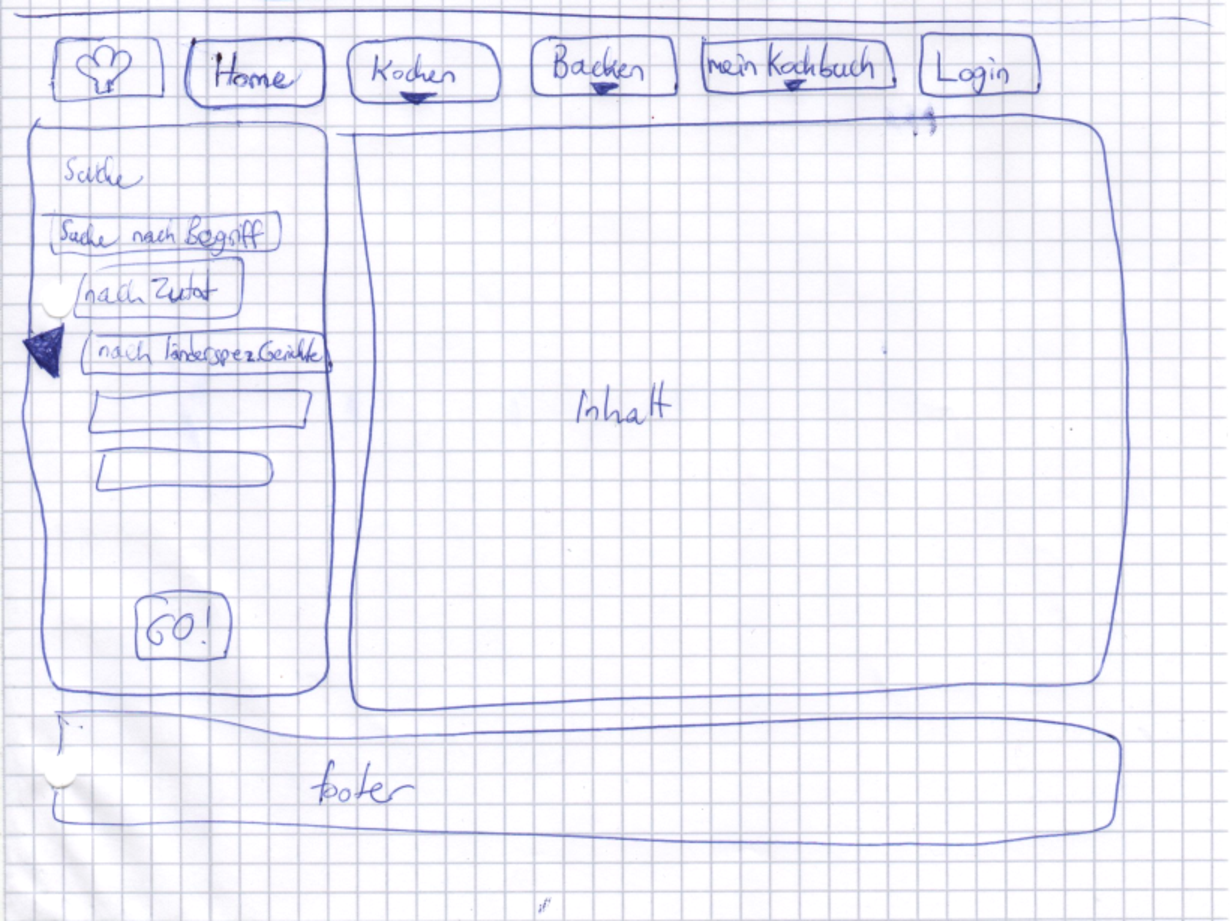
\includegraphics[scale=0.8]{Entwürfe/velat2.pdf}


\textbf{Vorteile:}\\
- seitlicher Suchbereich: Kategorien können aus- und eingeklappt werden: übersichtlich\\
- mehr Platz für Inhalt, da Suchbereich verborgen werden kann.

\textbf{Nachteile:}\\
- Im Dropdownmenü ist persönl. Bereich schon enthalten, obwohl noch nicht eingeloggt.

\newpage
% ------------------------------------------------------------------------------------
\section*{Entwurf 5} % Tamar 1

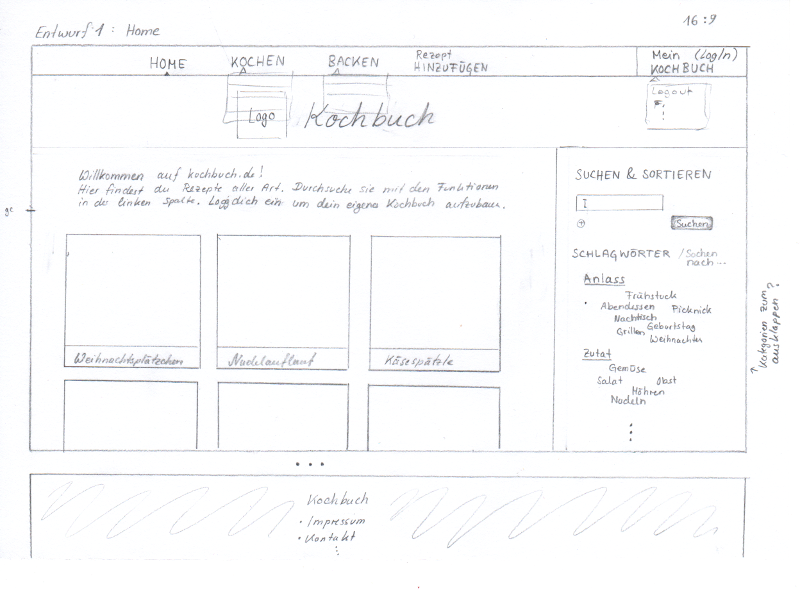
\includegraphics[scale=1]{Entwürfe/tamar1_1.png}\\
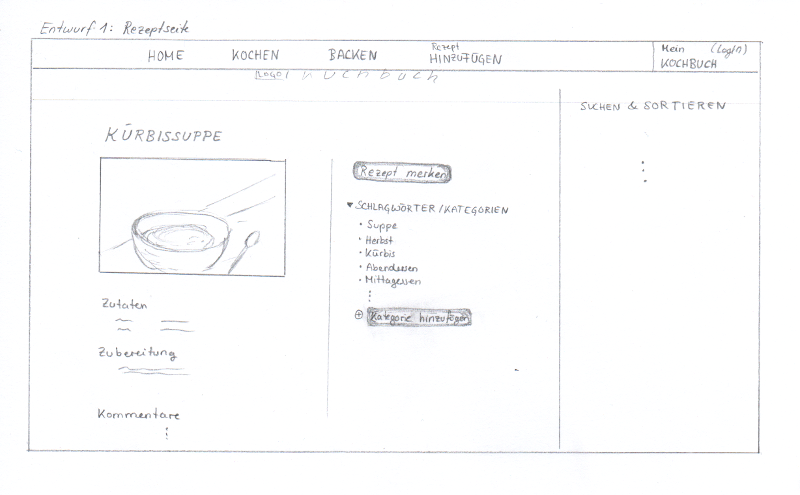
\includegraphics[scale=1]{Entwürfe/tamar1_2.png}
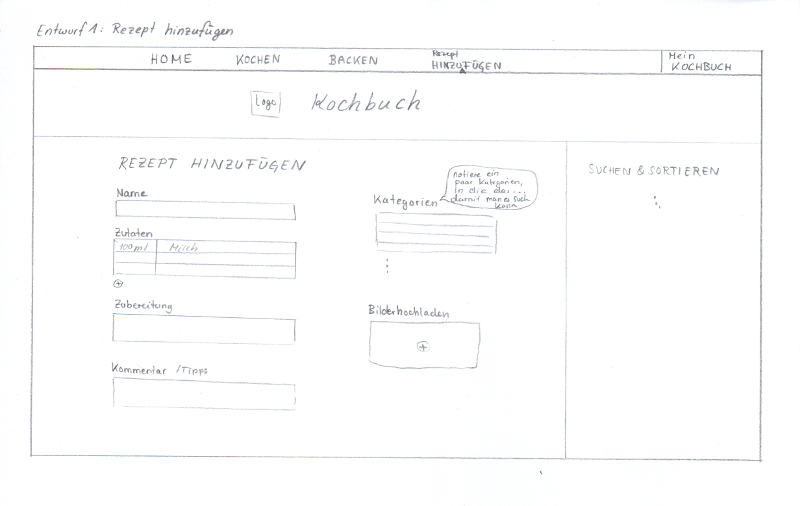
\includegraphics[scale=1]{Entwürfe/tamar1_3.png}



\textbf{Vorteile:}\\
- klassischer Aufbau\\
- Suche jederzeit sichtbar\\
- übersichtlich

\textbf{Nachteile:}\\
- Rezept hinzufügen sollte unter mein Kochbuch kommen, da es sonst nicht in die Navigationsstruktur passt\\
- Suchfunktion verbraucht Platz\\
- auf Rezeptseite muss Rezept mehr Platz einnehmen
\newpage
% ------------------------------------------------------------------------------------
\section*{Entwurf 6} % Tamar 2

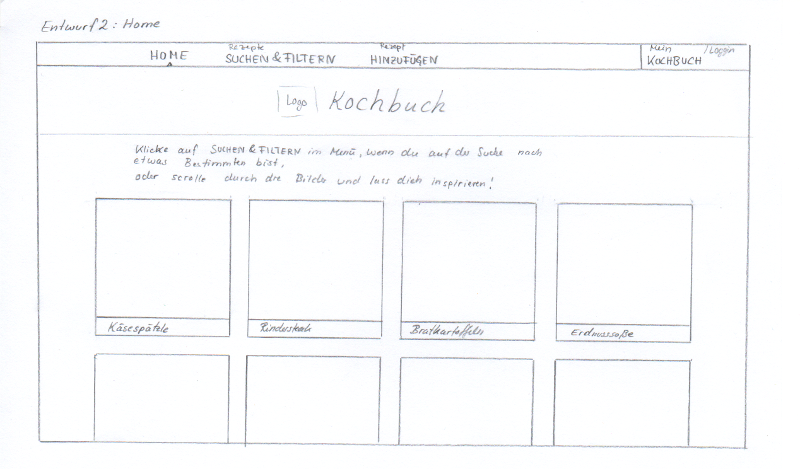
\includegraphics[scale=1]{Entwürfe/tamar2_1.png}
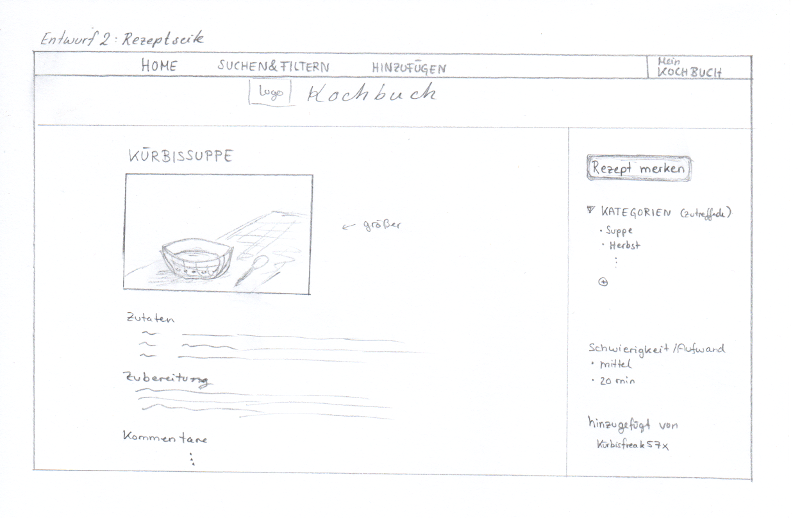
\includegraphics[scale=1]{Entwürfe/tamar2_2.png}\\
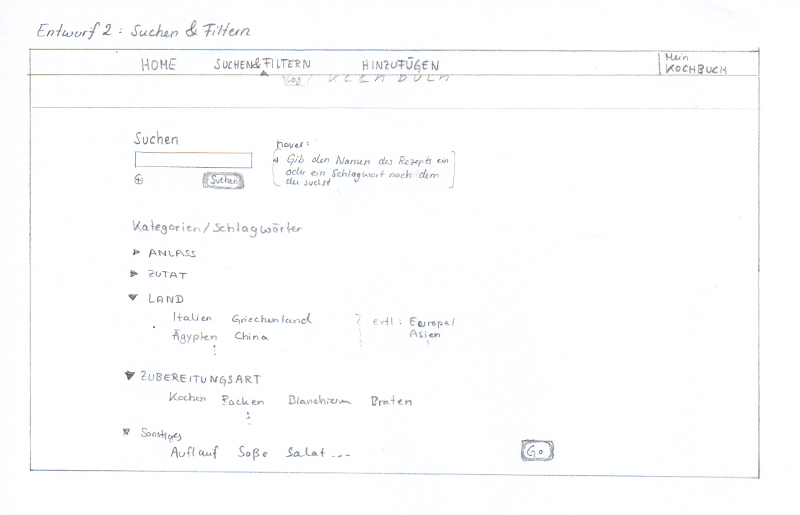
\includegraphics[scale=1]{Entwürfe/tamar2_31.png}
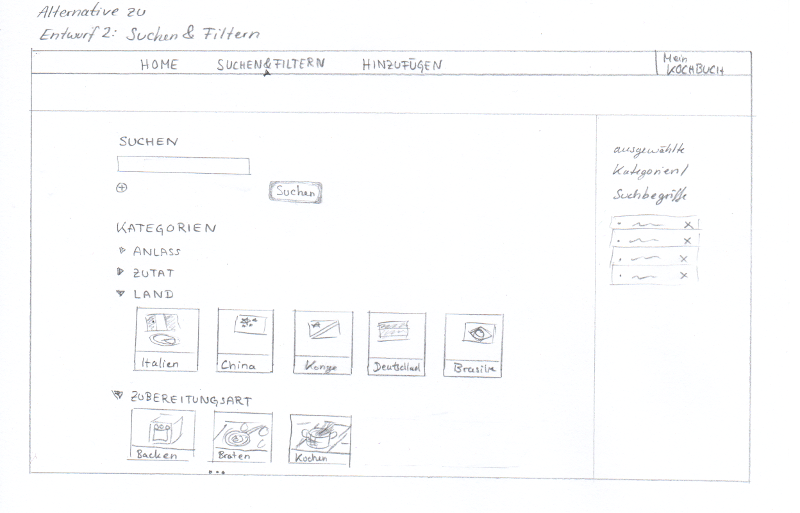
\includegraphics[scale=1]{Entwürfe/tamar2_32.png}


\textbf{Vorteile:} \\
- mehr Platz\\
- aufgeräumter

\textbf{Nachteile:}\\
- Suche als eigene Seite hat Nachteil, dass man ausgewählte Kategorien nicht nebenher sieht.\\
- Suchseite zu überladen


\pagebreak
% ------------------------------------------------------------------------------------
\section*{Planung des Prototypen}

\begin{enumerate}
 \item möglichst übersichtliches, klassisches Design um intuitives Zurechtfinden zu ermöglichen (rechts oben Login)
 \item Navigation aufgespalten:
 \begin{itemize}
  \item einerseits: horizontale Navigation stellt organisatorisches dar: Meta-Navigation, wie Home und Profilverwaltung / persönlicher Bereich
  \item andererseits: Seitenmenü enthält Kategorien, nach denen Rezepte sortiert/gefiltert werden können. Für Nutzer, die genau wissen was sie wollen, gibt es die Suchleiste.
 \end{itemize}
 \item Navigation und Struktur der Webseite ist für den Nutzer ersichtlich, da auf jeder Seite Navigation an gleicher Stelle bleibt und sich eventuell dynamisch anpasst (checkboxen)
 \item Navigation nimmt nicht notwendigerweise zu viel Platz der Webseite ein, da sie eingeklappt/verborgen werden kann
 \item Damit das seitliche Menü ersichtlich bleibt, sind einzelne Kategorien (Kochen, Backen, usw.) eingeklappt. Nach Bedarf können diese ausgeklappt werden, damit Unterkategorien sichtbar sind. 
 \item Der Großteil des Seiteninhalts besteht aus Bildern von Rezepten und der dazugehörige Kochvorgang.

\end{enumerate}



\pagebreak
% ------------------------------------------------------------------------------------
% AUFGABE 4
% ------------------------------------------------------------------------------------
\section{Prototyp}


% ------------------------------------------------------------------------------------
\subsection*{Grundaufbau}

Startseite:
\begin{center}
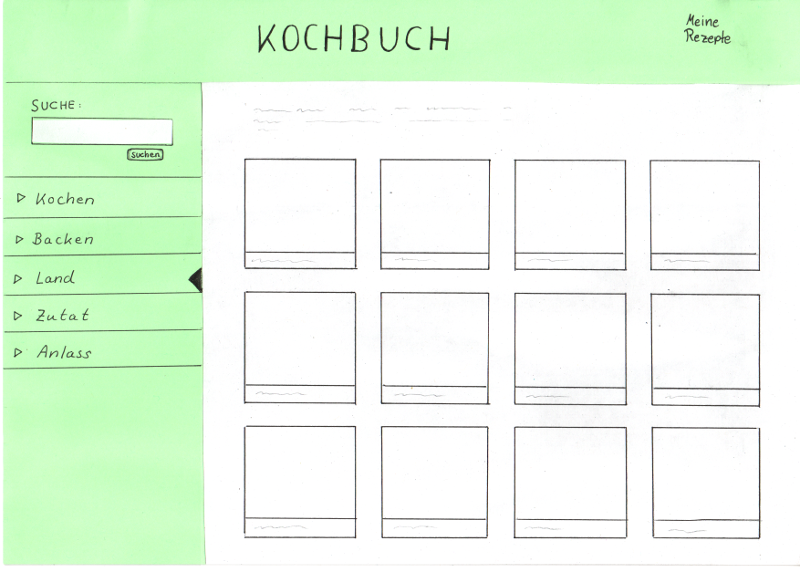
\includegraphics[scale=0.4]{Prototyp/home.png}
\end{center}

Die Startseite enthält einen kurzen Begrüßungstext mit einer kurzen Erklärung der Navigation und Bilder von verschiedenen Rezepten.\\
Rechts oben befindet sich der Menüpunkt der zum persönlichen Kochbuch bzw. Login führt.\\
Auf der linken Seite gibt es die Möglichkeit, die Rezepte nach Belieben zu filtern. Entweder nach Suchbegriffen oder nach verschiedenen Kategorien, die auf dem Prototypen in einer Auswahl dargestellt sind.

\pagebreak
Rezeptseite:
\begin{center}
\includegraphics[scale=0.4]{Prototyp/plätzchenrezeptseite.png}
\end{center}

Eine Rezeptseite enthält ein Bild, Zutaten, Zubereitung und Kommentare zu einem Rezept. In dem Bereich auf der rechten Seite befindet sich der Button, um das Rezept zu speichern. Ist man nicht eingeloggt, wird man aufgefordert, sich einzuloggen. 
Außerdem befinden sich auf der Seite Informationen zum Aufwand des Gerichtes und die Kategorie, in der es sich befindet. 

\pagebreak
% ------------------------------------------------------------------------------------
\subsection*{Funktionalität der Navigation}

Einklappen der Seitennavigation:
\begin{center}
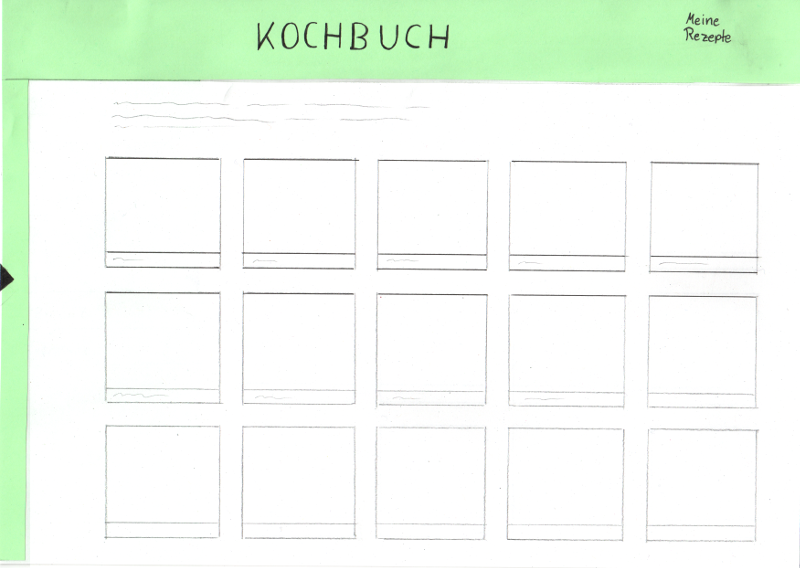
\includegraphics[scale=0.4]{Prototyp/home_menuhidden.png}
\end{center}

Die Seitennavigation kann durch Betätigung des Pfeiles auf der linken Seite ein- bzw. ausgeklappt werden. 

horizontales Menü: meine Rezepte
\begin{center}
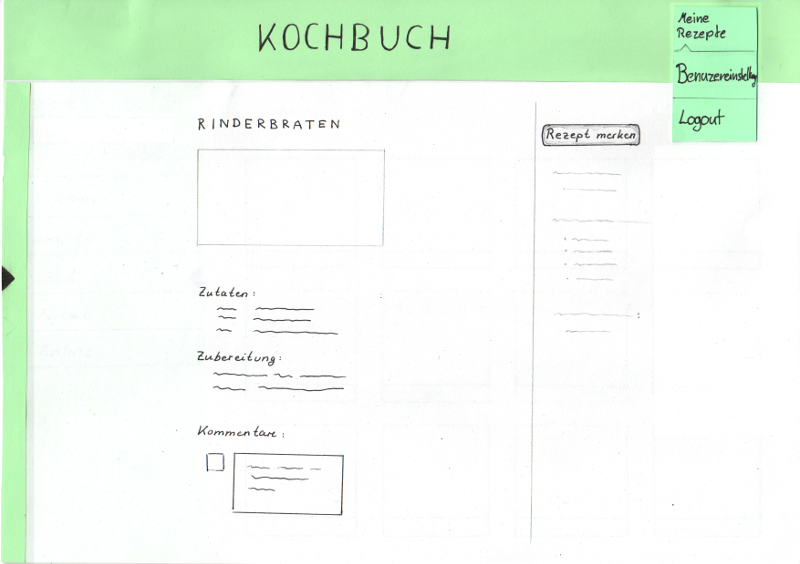
\includegraphics[scale=0.4]{Prototyp/menu_eigeneRezepte_menuhidden.png}
\end{center}


Die einzelnen Menüpunkte sind durch Anklicken des Pfeiles aufklappbar:

Menü: Kochen
\begin{center}
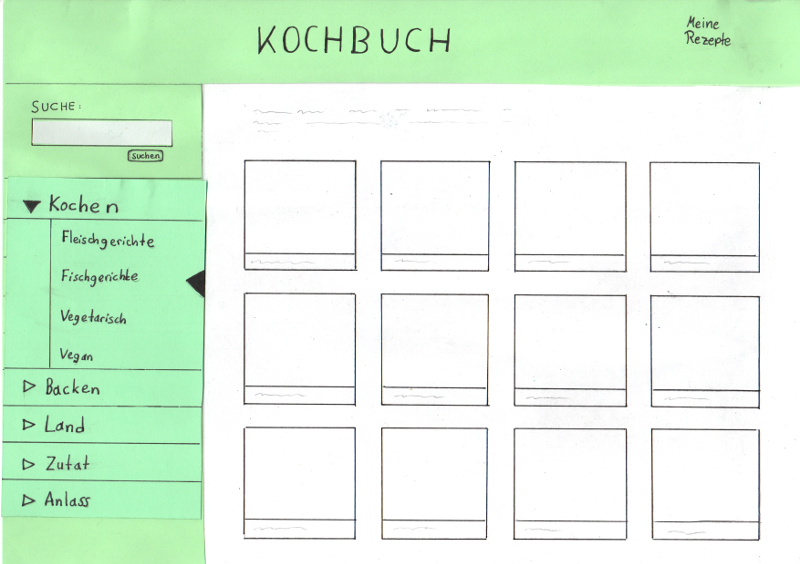
\includegraphics[scale=0.4]{Prototyp/menu_kochen.png}
\end{center}

Menü: Backen
\begin{center}
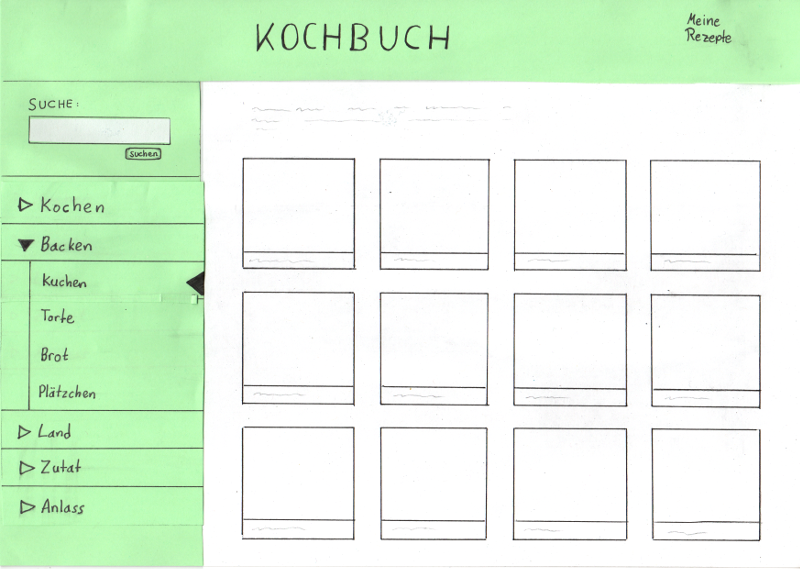
\includegraphics[scale=0.4]{Prototyp/menu_backen.png}
\end{center}
\newpage
Menü: Zutat
\begin{center}
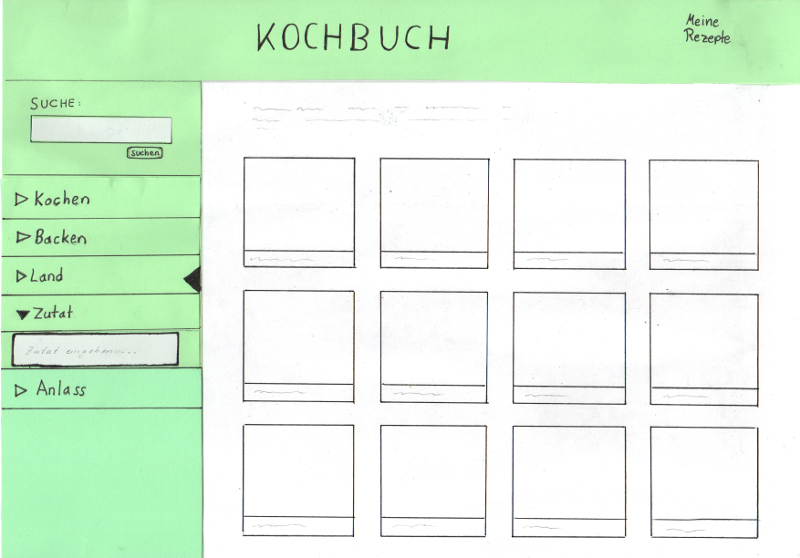
\includegraphics[scale=0.4]{Prototyp/menu_zutat.png}
\end{center}

\pagebreak
% ------------------------------------------------------------------------------------
\subsection*{Szenarien}

\subsubsection*{Szenario 1: Max will Plätzchen backen}

Er verwendet die Suchfunktion, gibt "Plätzchen" ein und erhält Plätzchenrezepte.
\begin{center}
\includegraphics[scale=0.4]{Prototyp/plätzchensuche.png}
\end{center}

Er wählt ein Rezept aus und wird auf die entsprechende Rezeptseite gebracht.
\begin{center}
\includegraphics[scale=0.4]{Prototyp/plätzchenrezeptseite.png}
\end{center}


\subsubsection*{Szenario 2: Karl hat nur bestimmte Zutaten da}

Er wählt im Seitenmenü "Zutat" aus...
\begin{center}
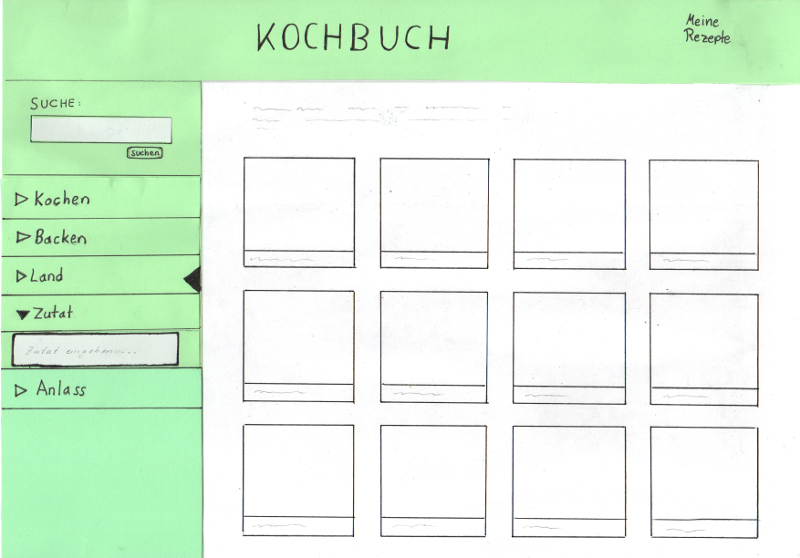
\includegraphics[scale=0.4]{Prototyp/menu_zutat.png}
\end{center}

... und gibt die Zutaten ein, die ihm zur Verfügung stehen: Nudeln, Hackfleisch und Tomaten
\begin{center}
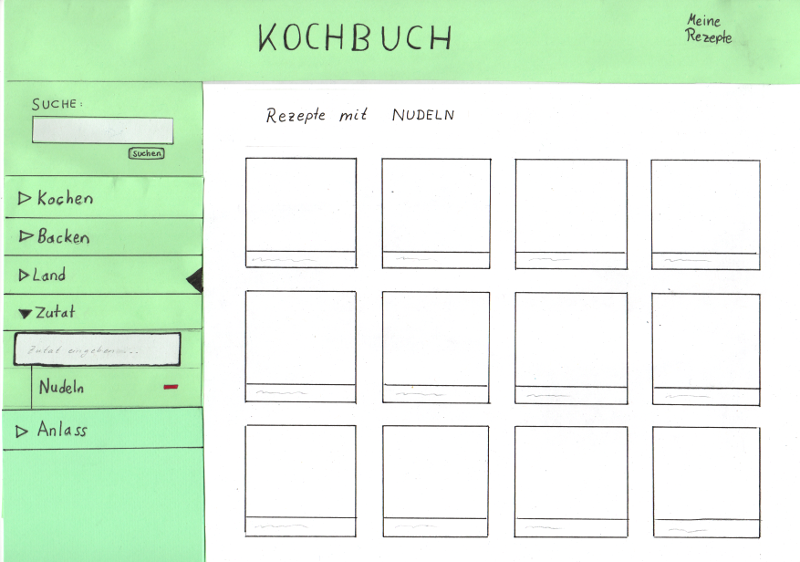
\includegraphics[scale=0.4]{Prototyp/menu_zutat_nudeln.png}\\[1em]
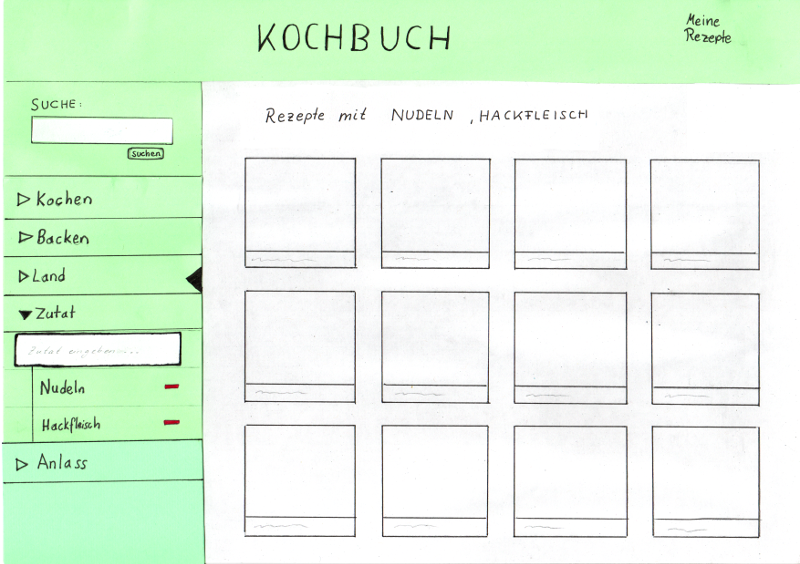
\includegraphics[scale=0.4]{Prototyp/menu_zutat_nudelnhackfleisch.png}\\[1em]
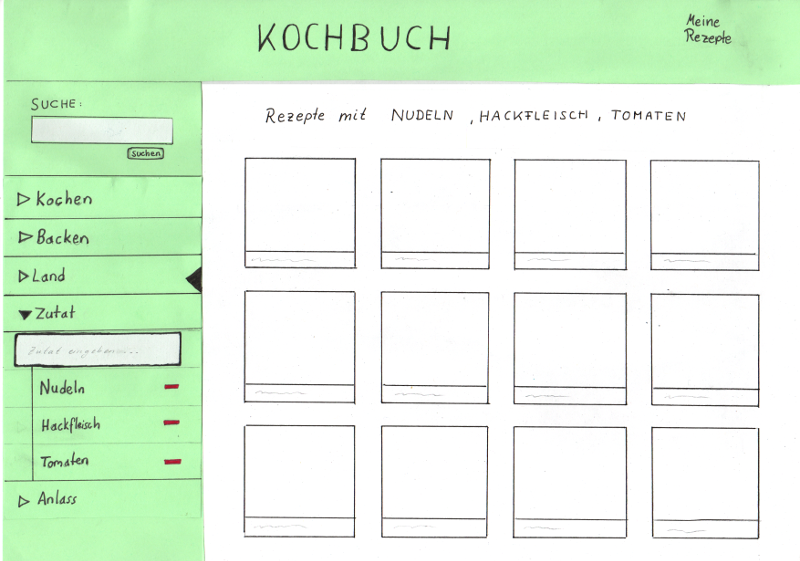
\includegraphics[scale=0.4]{Prototyp/menu_zutat_nudelnhackfleischtomate.png}
\end{center}
Er bekommt eine Auswahl von Rezepten, die zu seinen Zutaten passen.

\pagebreak
\subsubsection*{Szenario 3: Anna lässt sich inspirieren}

Anna klappt das Seitenmenü ein, um auf der gesamten Breite die Bilder der Rezepte betrachten zu können.
\begin{center}
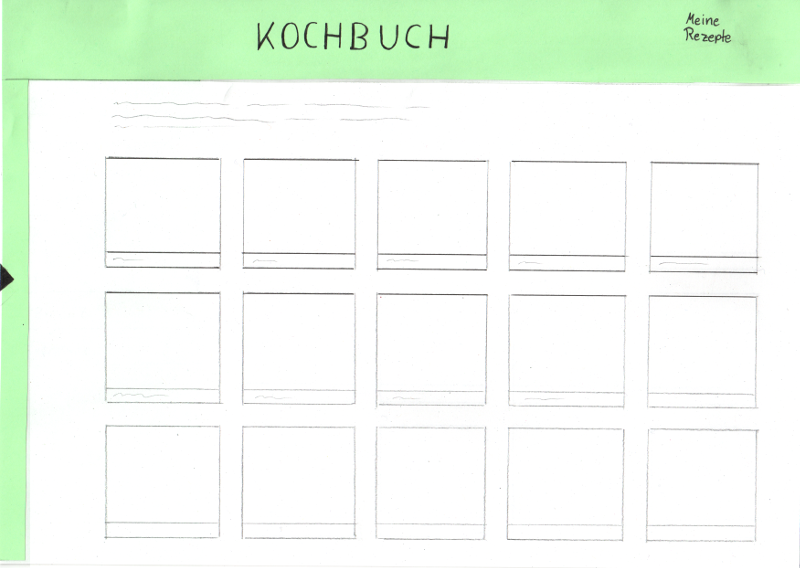
\includegraphics[scale=0.4]{Prototyp/home_menuhidden.png}
\end{center}

Sie scrollt durch die Bilder und sieht sich ein bestimmtes Rezept an.
\begin{center}
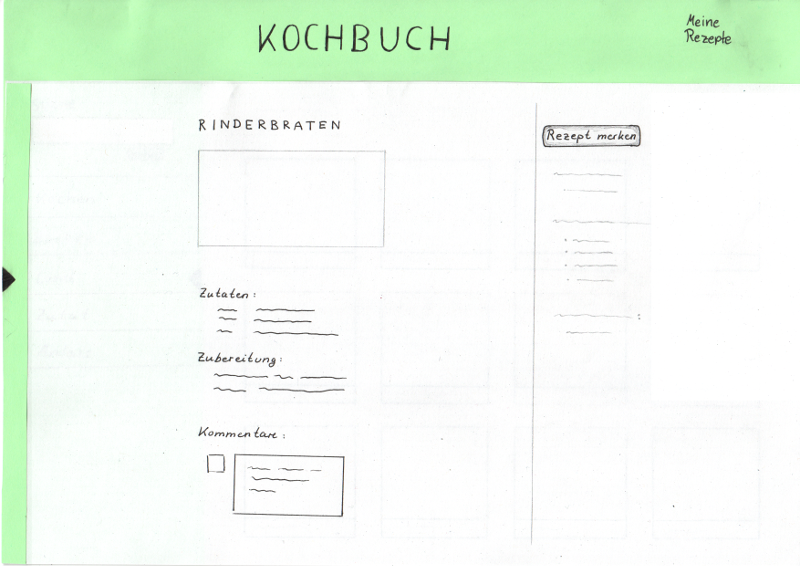
\includegraphics[scale=0.4]{Prototyp/rezeptseite_menuhidden.png}
\end{center}

Sie klickt auf "Rezept merken" und sieht sich dann unter "meine Rezepte" ihre bisher gespeicherten Rezepte an.
\begin{center}
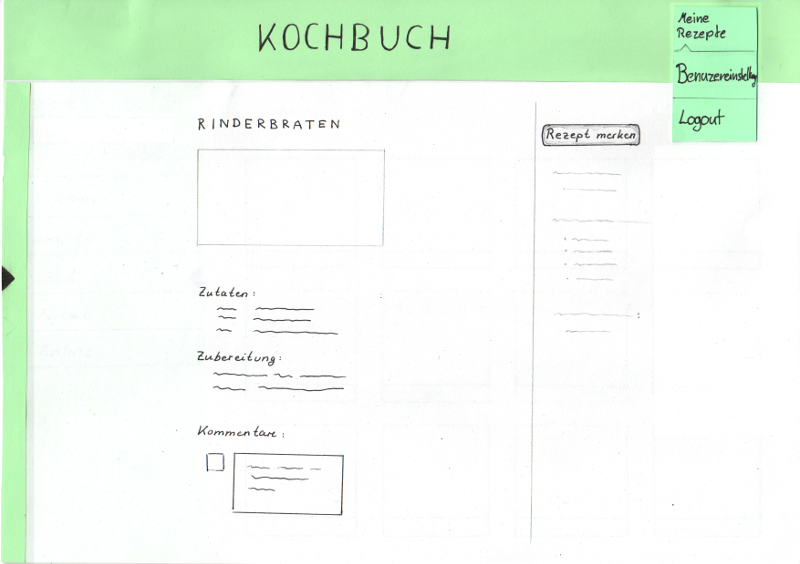
\includegraphics[scale=0.4]{Prototyp/menu_eigeneRezepte_menuhidden.png}\\[1em]
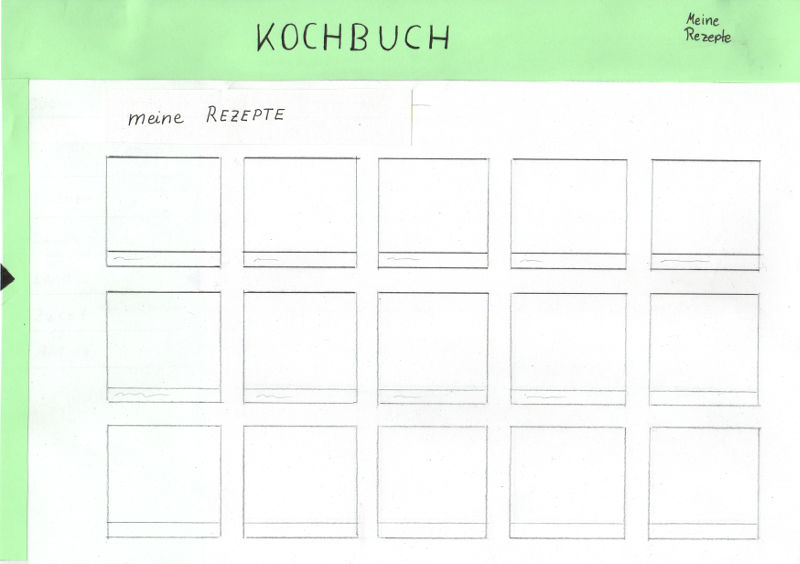
\includegraphics[scale=0.4]{Prototyp/meineRezepte_menuhidden.png}
\end{center}



% ------------------------------------------------------------------------------------
% AUFGABE 5
% ------------------------------------------------------------------------------------
%\section{Präsentation}
\stepcounter{section}
\newpage
% ------------------------------------------------------------------------------------
% AUFGABE 6
% ------------------------------------------------------------------------------------
\section{Heuristische Evaluation}

\subsection*{a) Durchführung}

\subsubsection*{1. Heuristiken}

\textbf{Kontingenz, Kontinuierlichkeit und Standards}\\
Der Aufbau der Seite, sowie die wichtigsten Begriffe, bleiben über verschiedene Unterseiten hinweg konstant

\textbf{die Navigation ist intuitiv und verständlich}\\
Die wichtigsten Funktionen können schnell gefunden werden. Die Navigationspunkte und Begriffe sind eindeutig und verständlich. Benutzer sehen, wo sie sich innerhalb der Struktur der Webseite befinden.

\textbf{Rückmeldungen \& Sichtbarkeit des Systemstatus}\\
Für Aktionen erhält der Nutzer eine Rückmeldung und weiß, was seine Aktion bewirkt hat. Der Nutzer sieht den Status den Systems, beispielsweise ob er eingeloggt ist.

\textbf{Kontrolle und Freiheit}\\
Der Nutzer kann die Navigation so verwenden, wie er sie versteht und auf verschiedenen Wegen zu seinem Ziel gelangen.

\textbf{Die Benutzeroberfläche ist visuell ansprechend}\\
Der Benutzer fühlt sich auf der Webseite wohl und die Gestaltung passt dazu, was die Seite inhaltlich bietet.

% --------------------------------------------------------
% Heuristische Evaluation
% --------------------------------------------------------
\subsubsection*{2. Heuristische Evaluation: Protokolle}

\hrulefill\\
% --------------------------------------------------------
% Protokoll: Chris
% --------------------------------------------------------
\textbf{Chris}\\
\begin{itemize}
\item \textbf{Kontingenz und Standards}\\    
Ist gegeben, da die Navigation immer an der selben Stelle bleibt in genau der gleichen Größe.
Auch der Hauptinhalt bleibt gleich groß und an der selben Stelle,
Genauso wie der obere Frame an dem sich nichts ändert während man sich auf der Seite umschaut.

\item \textbf{Intuitiv und verständlich}\\  
Da sich der Prototyp sich vom Designe an den meisten Webseiten orientiert, gerade was Navigation und Aufbau betrifft ist ein intuitive Handhabung gegeben.
Rückmeldung und Sichtbarkeit des Sichtbarkeit des Systemstatus
Ist nur bedingt gegeben bei Standartaktionen ist klar ersichtlich was passiert doch bei unerwarteten eingaben oder bei fehlerhaften Suchanfragen ist noch nicht ersichtlich was passiert, oder ob es zu einer Fehlermeldung kommt.
Auch bei einem falschen Login oder überhaupt beim Login ist noch nichts ersichtlich.

\item \textbf{Kontrolle und Freiheit}\\ 
Der Benutzer kann jederzeit frei und ohne Einschränkung Navigieren, allerdings ist es noch nicht ersichtlich ob man auf verschiedene Art und Weise zu den gleichen Seiten kommt aber durchaus vorstellbar, einerseits durch die Suche anderseits durch das linke Menü.

\item \textbf{Visuell ansprechend}\\ 
Der Prototyp ist zwar farblich gestaltet, aber weder Logo noch einpassender Name ist gewählt.
Auch inhaltlich ist noch nicht viel geboten es liegen gute Ansätze vor diese jedoch erst noch umgesetzt werden müssen.
\end{itemize}
\hrulefill\\

% --------------------------------------------------------
% Protokoll: Velat
% --------------------------------------------------------
\textbf{Velat}\\
\begin{itemize}
\item \textbf{intuitive und verständliche Navigation}\\ 
Es existiert kein "Home-Button", durch den man von überall auf eine Startseite gelangt (die übrigens auch nicht existiert)
Es gibt nur eine Seite, auf der zufällige Gerichte angezeigt werden. Ist diese Seite nur am Anfang des Besuches sichtbar?

\item \textbf{visuell ansprechend}\\
Gibt es einen Namen für die Webseite? Das zentrierte "Kochbuch" im Header ist nicht unbedingt sehr einfallsreich und sollte durch einen Namen bzw. ein Logo ersetzt werden, der auch an einer besseren Stelle platziert sein sollte. 

\item \textbf{intuitive und verständliche Navigation}\\
Menüpunkt "Land" verwirrt (Vorschlag: länderspezifisch / International).          
Menüpunkt "Zutat" besser beschreiben. Nutzer weiß nicht genau, was unter diesem Punkt zu finden ist.
(Vorschlag: in "Zutat eingeben" umbenennen oder direkt in Form einer Suchleiste im Menü unterbringen...)


\item \textbf{visuell ansprechend}\\
Unter eigene Rezepte:
\begin{enumerate}[o]
\item  Einklapp-Funktion\\
Zutaten, Zubereitung und Kommentare sind zentriert. 
Warum also die Einklapp-Funktion d. Menüs ?
(Vorschlag: Wenn durch die Einklapp-Funktion des Menüs Platz gespart werden soll, sollte der Inhalt links ausgerichtet sein.)
\item Hervorhebung\\
Zumindest der Button "Rezept merken" muss hervorgehoben werden. 
(Vorschlag: z.B. durch Farbe $\rightarrow$ gelb/rot?) 
\end{enumerate}

\item \textbf{Rückmeldungen und Sichtbarkeit des Systemstatus}\\
Eine Fehlermeldung muss ausgegeben werden, falls die Suche nicht erfolgreich sein sollte.

\end{itemize}
\hrulefill\\
% --------------------------------------------------------
% Protokoll: Tamar
% --------------------------------------------------------
\textbf{Tamar}
\begin{itemize}
 \item \textbf{Kontingenz, Kontinuierlichkeit und Standards}\\
 Beobachtungen beim Navigieren durch alle Seiten des Prototypen:\\
 Hauptaufbau ist auf jeder Seite gleich.\\
 Darstellung der Rezeptauswahl bleibt konstant über Seiten hinweg.\\
 Navigationselemente und Filter/Suche sind von überall aus erreichbar, auch von den Rezeptseiten.\\
 Seitenaufbau hält sich an bekannte Standards.\\
 Suchbegriffe und ausgewählte Filterbegriffe sollten.\\
 Die Suchauswahl und Auswahl von Filterbegriffen sollte ausgewählt bleiben, auch wenn verschiedene Unterseiten besucht werden - die volle Funktionalität ohne JavaScript und Datenbanken umzusetzen, ist nicht möglich, aber auf statische Weise sollte es trotzdem umgesetzt werden.
 
 \item \textbf{die Navigation ist intuitiv und verständlich}\\
 Startseite: oben Login und seitliche Navigation für die Rezepte ist eine verständliche, beziehungsweise gewohnte Anordnung. (Seitenleiste zur Filtersuche vergleichbar mit Amazon)\\
 Art und Weise des Filterns/Suchens ist somit auch intuitiv/verständlich\\
 Navigationsleiste:\\
 Reihenfolge der Begriffe nicht so, wie man es erwarten würde.\\
 Was exakt unter Kochen und was unter Backen einzuordnen/zu erwarten ist, ist nicht unbedingt für alle gleich. Manche Nutzer würden unten Backen hauptsächlich Süßes und Gebäck erwarten, andere aber auch Aufläufe, Rinderbraten und ähnliches.\\
 Ersichtlicher wäre eine Aufteilung in Herzhaft und Süß.\\
 Einordnung nach Fisch/Fleisch sollte extra zu finden sein.\\
 Aufteilung könnte man an Standardkochbücher anpassen und Überbegriff verwenden wie: Zubereitungsart (darunter: Kochen, Backen, Braten usw.)

 \item \textbf{Rückmeldungen \& Sichtbarkeit des Systemstatus}\\
 Ob man eingeloggt ist oder nicht, sieht man nicht auf den ersten Blick.\\
 Ebenso: ob man gerade alle Rezepte durchsucht oder nur diejenigen, die im eigenen Kochbuch gespeichert sind ist nicht sichtbar.\\
 Es sollte eine Rückmeldung geben, wenn man ein Rezept zum eigenen Rezeptbuch hinzugefügt/entfernt hat.\\
 In der Seitennavigation sollte jederzeit sichtbar sein, was aktuell ausgewählt ist und nach welchen Suchbegriffen gesucht wird. Über der angezeigten Auswahl von Rezepten wird angezeigt, wonach gerade gefiltert wird, aber von einer einzelnen Rezeptseite aus, sollte man es auch in der Seitenleiste sehen.

 \item \textbf{Kontrolle und Freiheit}\\
 Bei der Durchsuchung/Filterung der Rezepte hat der Nutzer alle Freiheiten. Er kann beliebiges auswählen und die Auswahl wieder rückgängig machen. Der Nutzer kann die Navigation so verwenden wie er sie versteht und für seine Zwecke gebrauchen kann. Der Nutzer kann auch auf verschiedenen Wegen zum gleichen Rezept gelangen.

 \item \textbf{Die Benutzeroberfläche ist visuell ansprechend}\\
 Das Design lenkt nicht vom dargestellten Inhalt der Seite ab, sondern stellt den Inhalt - die Rezepte - in den Mittelpunkt.\\
 In der Übersicht sind in erster Linie die Bilder der Rezepte zu sehen, was die Athmosphäre der Seite an den Inhalt anpasst.\\
 Rezeptseite: Hat viel Whitespace. Bild sollte größer sein.

\item \textbf{resultierende Probleme:}
\begin{enumerate}[o]
 \item Oberbegriffe in Seitennavigation: nicht intuitiv und für alle Nutzer gleichermaßen vertändlich, welche Kategorie wo zu finden ist\\
(Vorschlag: filtern nach... \\
 - Anlass oder Art (süß, herzhaft, Frühstück, Mittag, Picknick, Snack, Getränke) \\
 - Ernährungsweise (vegan, vegetarisch, glutenfrei, gesund) \\
 - Land (griechisch, italienisch, ...) \\
 - Zutat [Eingabefeld] \\
 - Zubereitungsart (Kochen, Backen, Braten) \\
 - Hauptzutat (Fleisch, Fisch, Gemüse, Obst)

\item nicht ersichtlich, ob man gerade eingeloggt ist, oder nicht\\

\item nicht ersichtlich, ob gerade nur eigene Rezepte oder alle durchsucht werden\\
(Vorschlag: extra Punkt in Seitennavigation (vgl. Amazon) Ergebnisse anzeigen für: eigene Rezepte/alle Rezepte)

\item Auswahl von Filterbegriffen beibehalten (Schwierigkeit ohne JavaScript)

\item Rückmeldung geben für Aktionen: Rezept merken, Kommentar hinzugefügt
\item Rezeptseite ansprechender gestalten
\end{enumerate}
\end{itemize}
\hrulefill


% --------------------------------------------------------
% Probleme und Schwächen: Prioritäten
% --------------------------------------------------------
\subsubsection*{3. Probleme und Schwächen: nach Prioritäten geordnet}


\textbf{Priorität 1: Überarbeiten der Navigation}
\begin{enumerate}[\sbt]
 \item Home-Button-Funktion:\\
 Die Webseite hat keinen Home-Button und keine normale Startseite. Stattdessen gibt es die Rezeptübersichtsseite im ungefilterten Status. Der Nutzer sollte die Möglichkeit haben, immer auf eine solche Startseite zu gelangen.
 \item Filterbegriffe:\\
 Die existierenden Begriffe in der Seitennavigation und ihre Reihenfolge sind nicht verständlich und intuitiv. Die Filterkategorie „Zutat“ ist anders als die anderen, da sie ein Eingabefeld hat. Daher sollte es nicht inmitten der anderen Kategorien auftauchen.\\
\end{enumerate}

\textbf{Priorität 2: visuell ansprechende Gestaltung}\\
\textit{Dieser Punkt ist für uns so wichtig, da die Webseite stark davon abhängig ist, wie wohl sich Nutzer hier fühlen}
\begin{enumerate}[\sbt]
 \item Name der Webseite:\\
 Nur das Wort „Kochbuch“ im Header ist langweilig. Sollte durch ein Logo ersetzt werden.
 \item Einklappfunktion des Seitenmenüs:\\
 Vorallem bei der Ansicht einer Rezeptseite macht das eingeklappte Menü die Seite nicht schöner. Die Einklappfunktion schätzen wir daher als unwichtig ein.
 \item erkennbare Buttons:\\
 Wichtige Butten wie „Rezept merken“ müssen hervorgehoben sein\\
\end{enumerate}

\textbf{Priorität 3: Kontinuierlichkeit und Systemstatus}
\begin{enumerate}[\sbt]
 \item Sichtbarkeit fehlt:\\
 - ob man eingeloggt/ausgeloggt ist,\\
 - ob man gerade alle Rezepte oder nur die eigenen durchsucht
 \item Die Auswahl der Filterbegriffe sollte beibehalten werden, wenn zu einer anderen Unterseite gewechselt wird.\\
\end{enumerate}

\textbf{Priorität 4: Rückmeldung und Systemstatus}
\begin{enumerate}[\sbt]
 \item Fehlermeldung, wenn zu den gewählten Filterbegriffen keine Rezepte gefunden wurden
 \item Rückmeldungen für bestimmte Aktionen: Rezept merken, Kommentar hinzufügen
\end{enumerate}

% --------------------------------------------------------
% Problemlösungen
% --------------------------------------------------------
\subsubsection*{4. Problemlösungen}

\textbf{zu Priorität 1: Überarbeiten der Navigation}

Aubau des Seitenmenüs:\\[-3em]
\begin{addmargin}[25pt]{0pt}
>> Home-Button\\[0.4em]
>> Suche\\
>> Zutat\\[0.4em]
>> Zubereitungsart\\
>> Hauptzutat\\[0.4em]
>> Anlass\\
>> Land\\[0.4em]
>> Ernährungsweise\\
\end{addmargin}

\textbf{zu Priorität 2: visuell ansprechende Gestaltung}

\begin{enumerate}[$\to$]
 \item Logo in Header einbauen\\[-2.5em]
 \item Die Einklappfunktion des Seitenmenüs spielt keine tragende Rolle. Auch nicht für die visuelle Gestaltung der Seite: kann daher vernachlässigt werden\\[-2.5em]
 \item wichtige Buttons müssen hervorgehoben werden (Rezept merken)\\
\end{enumerate}


\textbf{Priorität 3: Kontinuierlichkeit und Systemstatus}\\
\textit{Alle Probleme dieser Kategorie sind für uns sehr schwer umzusetzen ohne die Verwendung von JavaScript. Daher müssen wir uns hier besonders überlegen, wie wir die Webseite trotzdem so aussehen lassen, dass die Punkte nicht ganz vernachlässigt werden}

$\to$ Notlösung: wenn die Webseite fertig gestaltet ist, werden alle Seiten kopiert, so dass sie einmal für den eingeloggten Zustand und einmal für den ausgeloggten existieren. Das gleiche kann man für die Auswahl der Filterbegriffe machen. Das stellt sich aber vermutlich als zu aufwändig heraus, kann aber stellvertretend für einen Filterbegriff umgesetzt werden.\\

\textbf{Priorität 4: Rückmeldung und Systemstatus}

\begin{enumerate}[$\to$]
 \item Wenn keine Rezepte zur Filterauswahl gefunden werden, wird an der Stelle eine Fehlermeldung gezeigt, an der sonst die Rezepte erscheinen würden. „Es wurden leider keine Rezepte gefunden, (die zu allen ausgewählten Kategorien gehören)".\\[-2.5em]
 \item für das Hinzufügen eines Kommentars ist keine anschließende Erfolgsmeldung nötig, da der Nutzer sehen kann, wenn der Kommentar neu erscheint.\\[-2.5em]
 \item Nach dem Merken eines Rezepts erscheint eine Meldung: „Das Rezept wurde in deinem Kochbuch gespeichert“.\\
\end{enumerate}

\subsection*{b) Änderungen}
Bei der Umsetzung der Webseite werden aufgrund der heuristischen Evaluation folgende Änderungen am Prototypen vorgenommen:
\begin{enumerate}[\sbt]
 \item Das Seitenmenü wird inhaltlich fast komplett überarbeitet. Die Reihenfolge und Bezeichnung für die Kategorien wird wie oben beschrieben angepasst. Es wird die Möglichkeit eingebaut, zu einer Art Startseite, beziehungsweise einer ungefilterten Anzeige aller Rezepte, zu gelangen. Außerdem kann der Nutzer im Seitenmenü wählen, ob er alle Rezepte oder nur die eigenen durchsuchen will. Letzteres ist nur möglich, wenn der Nutzer auch eingeloggt ist. Da die volle Funktionsweise des Seitenmenüs und der Buttons im Seitenmenü nur mit html und css kaum umsetzbar ist, wird die Auswahl von Filterkategorien nicht dynamisch funktionieren (dafür wäre ajax nötig). Stattdessen wird nach festgelegten Begriffen gefiltert, beziehungsweise gesucht.\\
 Um das ein- und ausloggen nachzuahmen, werden alle Seiten (auch die Rezeptseiten) für den eingeloggten sowie den ausgeloggten Zustand erstellt.\\
 Die Einklappfunktion des Seitenmenüs ignorieren wir bei der Umsetzung der Webseite, da es für die Nutzung und Gestaltung der Seite keine tragende Rolle spielt.

 \item Damit die Webseite für den Nutzer ansprechend und dem Thema angemessen ist, verwenden wir als Akzentfarbe ein frisches Grün und helle, warme Grautöne für große Flächen. Im Header wird ein Logo eingefügt. Buttons werden so gestaltet, dass sie schnell entdeckt werden und wie herkömmliche Buttons aussehen.
 
 \item Die Webseite gibt für wichtige Aktionen des Nutzers eine Rückmeldung. Werden Rezepte gefiltert, ist über den angezeigten Rezepten notiert, wonach gerade gefiltert wird. Wird auf „Rezept merken“ gedrückt, bekommt der Nutzer entweder den Hinweis, dass er sich einloggen muss, um diese Funktion zu verwenden, oder es erscheint die Meldung, dass das Rezept erfolgreich gespeichert wurde.\\
 Damit der Nutzer sehen kann, ob er eingeloggt ist oder nicht, wird der Menüpunkt „meine Rezepte“ jeweils angepasst. Ist der Nutzer ausgeloggt, kann er sich über diesen Menüpunkt einloggen. Ist er eingeloggt, findet er dort die Funktion sich auszuloggen oder zu seinen eigenen Rezepten zu gelangen.
\end{enumerate}


% ------------------------------------------------------------------------------------
% AUFGABE 7
% ------------------------------------------------------------------------------------
%\section{Umsetzung des Projekts}
\stepcounter{section}

% ------------------------------------------------------------------------------------
% AUFGABE 8
% ------------------------------------------------------------------------------------
\section{Prüfung der Barrierefreiheit}

% ------------------------------------------------------------------------------------
% AUFGABE 9
% ------------------------------------------------------------------------------------
\section{Nutzertest}
\textbf{Zielsetzung des Nutzertests}\\\\
 Kann die Webseite sinnvoll eingesetzt werden, um ein gewünschtes Rezept zu finden?
 
 Finden die User die Webseite angenehm gestaltet? Würden sie die Webseite gerne nutzen, wenn sie Rezepte suchen wollen?
 
 Verstehen die Nutzer, wie das Seitenmenü funktioniert und nutzen es so, wie wir uns vorgestellt haben, dass sie genutzt werden würde?
 
 Zwingen wir den Nutzer zu Denken oder ist die Webseite so gestaltet, dass sie für unsere Zielgruppe verständlich ist? 
 

\textbf{Auswertung}\\
\begin{enumerate}
\item Suche und Filter \\
- Suchfeld und Filter eindeutiger trennen\\
- Filter-Button zu weit unten. Man muss nach unten scrollen, damit man den Button sehen kann.\\
- Nach dem filtern: Seite scrollt/springt autom. nach ganz oben\\
\textcolor{red}{Priorität 1}

\item Unterschied: Auswahl zurücksetzen und Zurück zur Auswahl\\ 
- Unterschied zwischen den beiden Buttons ist unklar.\\
\textcolor{red}{Priorität 4}

\item Benutzerverwaltung \\
- Button Persönlicher Bereich passt nicht ins restliche Design der Webseite.\\
- Login fehlerhaft\\
- Auf den ersten Blick nicht genau erkennbar ob ein- oder ausgeloggt \\
\textcolor{orange}{Priorität 5}

\item Logo\\
- Logo ist nicht anklickbar bzw. ist nicht gleichzusetzen mit einem Home-Button. \\
\textcolor{green}{Priorität 6}

\item Hover-Effekte\\
- Namen der Rezepte erst sichtbar, wenn die Mauszeiger über dem Rezept ist. \\
\textcolor{green}{Priorität 7}

\item Platzhalter\\
- Es existieren noch Platzhalter.\\
\textcolor{green}{Priorität 7}
\end{enumerate}
\textbf{Lösungsvorschläge}\\
\begin{enumerate}
\item Suche und Filter \\
Um das Suchfeld und den Filter besser voneinander zu trennen, würde es sich anbieten, das Suchfeld direkt unterhalb des Headers zu platzieren. Dies wäre für die Übersichtlichkeit besonders von Vorteil (d.h. über "Auswahl zurücksetzen"). Eine andere und wirkungsvolle Variante wäre die, dass man das Suchfeld klassisch rechts oben platziert (jedoch würde dies nicht zu unseren Vorstellungen passen, da ja der Filterbereich links platziert ist). \\
Nachdem man den Filter bedient hat, springt/scrollt die Seite nach oben. Um dieses Problem einfach zu lösen, wäre es nötig, Gebrauch von JavaScript zu machen, was für dieses Projekt leider nicht möglich ist.\\
Damit der Filter-Button ohne zu Scrollen sichtbar ist, müsste man den Bereich an sich verkleinern.\\    
\item "Auswahl zurücksetzen" und "Zurück zur Auswahl"\\
Das Problem lässt sich sehr leicht beheben, in dem man "Zurück zur Auswahl" durch einen kleinen "Zurück"-Button ersetzt. \\ 
\end{enumerate}
\textbf{Bewertung}\\
Anhand der gemessenen Zeit und Anzahl der Klicks, die die Nutzer für die einzelnen Aufgaben gebraucht haben, lässt sich leicht erkennen, dass die Webseite einen übersichtlichen Aufbau hat. Die Nutzer hatten keine großen Schwierigkeiten, die Aufgaben zu lösen. Das Design ist laut Ergebnissen der Fragebögen gut ausgefallen und die Nutzer haben sich auf der Webseite ganz gut zurecht finden können. Mit etwas mehr Arbeit an einzelnen Buttons würden sich die Nutzer auf der Webseite noch wohler fühlen.\\
Im Großen und Ganzen ist die Webseite deutlich benutzerfreundlich, wenngleich man die wenigen kleinen Probleme mit mehr Zeitaufwand beheben könnte. 
% ------------------------------------------------------------------------------------
% AUFGABE 10
% ------------------------------------------------------------------------------------
\section{Projektabschluss}
\subsubsection*{Ausblick für Erweiterungsmöglichkeiten/Verbesserungen}
\textbf{Fehlende Inhalte/Funktionen}\\
Aufgrund der Beschränktheit unserer Arbeitsweise (nur HTML und CSS) gab es bestimmte Funktionen, die nicht implementiert werden konnten.
Eine dieser Funktionen ist das Einklappen der Navigation auf der linken Seite. Zudem ist das Anlegen eines neuen Benutzers nicht möglich, da wir keine Datenbank verwenden konnten. Eine andere Funktion, die nicht implementiert werden konnte, war die Suchfunktion. Das Kommentieren eines Rezeptes ist nur bedingt möglich (Textverfassung möglich, das Absenden nicht). \\\\
\textbf{Ausblick}\\
Für die Zukunft würde sich die Möglichkeit anbieten, unter Verwendung von Skriptsprachen (PHP, JS, ...) die fehlenden Funktionen zu implementieren. Neben der Überarbeitung von fehlerhafte Funktionen wie z.B. die Filterfunktion, könnte man den Code der Webseite viel effizienter gestalten und redundantes entfernen. Dadurch wäre es auch möglich eine Benutzerverwaltung anzulegen, da das Arbeiten mit einer Datenbank diese Art von Funktion unterstützt.    
Auch das Gestalten der Einklapp-Funktion der Navigation würde sich als einfach erweisen. 
Die Überlegung eine Slide-Funktion zu den Bildern der einzelnen Rezepten einzuführen würde sich im Bereich des möglichen befinden und gleichzeitig das Design der Webseite moderner gestalten. 
\subsubsection*{Arbeitsaufteilung}
Im ersten Teil des Projektes haben sich die Gruppenmitglieder getroffen und gemeinsam die Aufgaben bewältigt. Erst im zweiten Teil war eine Aufteilung der Arbeit nötig, nachdem die Gruppe gemeinsam die Heuristiken festgelegt und jeweils Evaluationen durchgeführt hat. Hierfür hat sich die Gruppe wieder getroffen und eine Aufgabenverteilung vorgenommen. Die Verteilung der Aufgaben sieht folgendermaßen aus:
\begin{enumerate}[o]
 \item Tamar\\
 Heuristikenevaluation\\
 Heuristiken und Dokumentation zu Aufgabe 6b\\
 Entwurf eines Logos\\
 Implementierung der ersten Version der Webseite\\
 Implementierung von Rezeptseiten\\
 Durchführung von Nutzertests als Protokollantin und Versuchsleiterin
 \item Velat\\
 Heuristikenevaluation\\
 Implementierung von Rezeptseiten\\
 Entwurf und Auswertung des Nutzertests\\
 Durchführung von Nutzertests als Protokollant und Versuchsleiter\\
 Bearbeitung der Aufgabe 10\\
 \item Chris\\
 Heuristikenevaluation\\
 Implementierung von Rezeptseiten\\
 Prüfung der Barrierefreiheit\\ 
 Durchführung von Nutzertests als Protokollant und Versuchsleiter\\
 Bearbeitung der Aufgabe 10\\
\end{enumerate}
 Die Aufgaben waren im Großen und Ganzen gerecht verteilt. Jedes Teammitglied hatte ungefähr denselben Arbeitsaufwand.
% ------------------------------------------------------------------------------------
% Anhang
% ------------------------------------------------------------------------------------
\pagenumbering{Roman}





\end{document}



